% Generated by paper/reproducibility/joint_failure_frontier.py.
% Required packages: tikz
% Required TikZ libraries: none
% Target width: 160 mm maximum
% Minimum text size: 9 pt
% Colour/greyscale intent: colour and greyscale
% All marks represent calculations from the finite simulator.
\begingroup
\definecolor{FailureMixed}{HTML}{215178}
\definecolor{FailureNoReject}{HTML}{8C4814}
\definecolor{FailureFamily}{HTML}{3A634D}
\definecolor{FailureFrozen}{HTML}{3C3C3C}
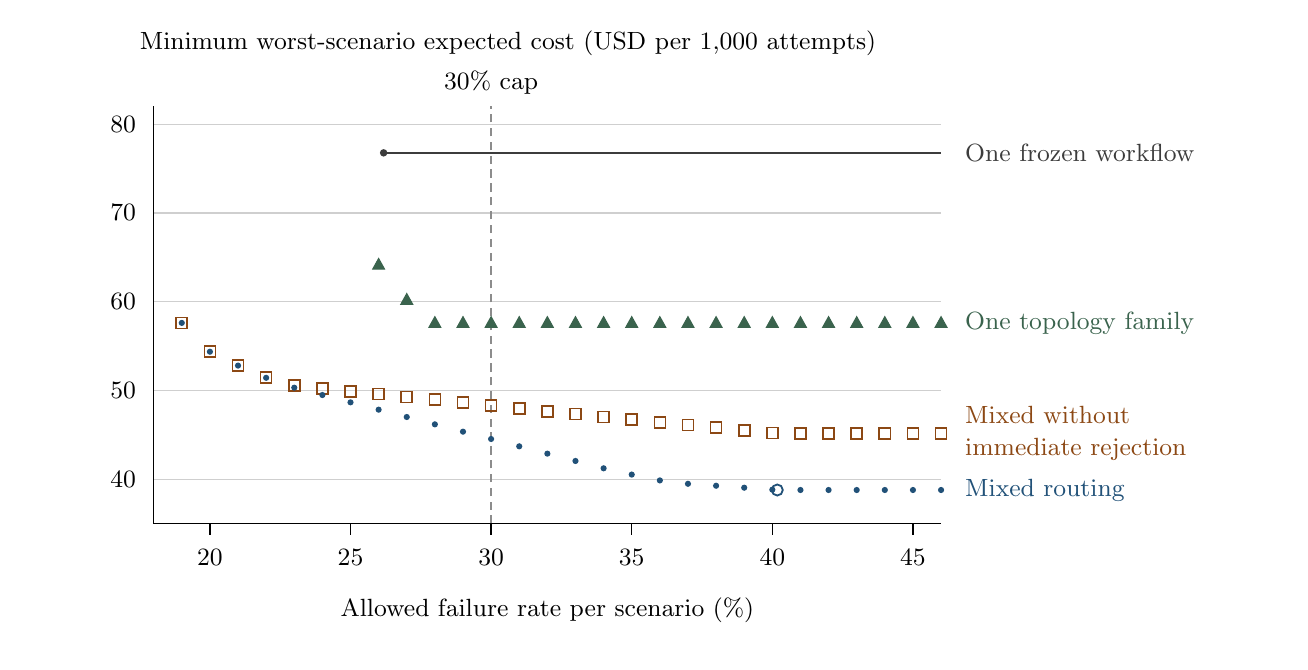
\begin{tikzpicture}[
  x=1mm,y=1mm,
  font=\fontsize{9.5}{11.5}\selectfont,
  axis/.style={line width=.5pt},
  grid/.style={draw=black!19,line width=.4pt},
  guide/.style={draw=black!45,line width=.5pt,densely dashed},
  family mark/.style={draw=FailureFamily,fill=FailureFamily,line width=.4pt},
  no reject mark/.style={draw=FailureNoReject,line width=.6pt},
  frozen step/.style={draw=FailureFrozen,line width=.65pt},
  direct/.style={anchor=west,align=left,inner sep=0pt},
]
\path[use as bounding box] (0,0) rectangle (159,78);

\draw[grid] (16,20.6383) -- (116,20.6383);
\node[anchor=east] at (15,20.6383) {40};
\draw[grid] (16,31.9149) -- (116,31.9149);
\node[anchor=east] at (15,31.9149) {50};
\draw[grid] (16,43.1915) -- (116,43.1915);
\node[anchor=east] at (15,43.1915) {60};
\draw[grid] (16,54.4681) -- (116,54.4681);
\node[anchor=east] at (15,54.4681) {70};
\draw[grid] (16,65.7447) -- (116,65.7447);
\node[anchor=east] at (15,65.7447) {80};
\draw[axis] (23.1429,15) -- (23.1429,13.6);
\node[anchor=north] at (23.1429,13) {20};
\draw[axis] (41.0000,15) -- (41.0000,13.6);
\node[anchor=north] at (41.0000,13) {25};
\draw[axis] (58.8571,15) -- (58.8571,13.6);
\node[anchor=north] at (58.8571,13) {30};
\draw[axis] (76.7143,15) -- (76.7143,13.6);
\node[anchor=north] at (76.7143,13) {35};
\draw[axis] (94.5714,15) -- (94.5714,13.6);
\node[anchor=north] at (94.5714,13) {40};
\draw[axis] (112.4286,15) -- (112.4286,13.6);
\node[anchor=north] at (112.4286,13) {45};
\draw[guide] (58.8571,15) -- (58.8571,68);
\node[anchor=south] at (58.8571,68.25) {30\% cap};
\draw[axis] (16,68) -- (16,15) -- (116,15);
\node[anchor=west] at (13,76) {Minimum worst-scenario expected cost (USD per 1,000 attempts)};
\node at (66,4) {Allowed failure rate per scenario (\%)};
\draw[frozen step] (45.2057,62.1023) -- (116.0000,62.1023);
\fill[FailureFrozen] (45.2057,62.1023) circle[radius=1.35pt];
\draw[no reject mark] (19.5714,40.5052) ++(-.7,-.7) rectangle ++(1.4,1.4);
\fill[FailureMixed] (19.5714,40.5052) circle[radius=1.12pt];
\draw[no reject mark] (23.1429,36.8464) ++(-.7,-.7) rectangle ++(1.4,1.4);
\fill[FailureMixed] (23.1429,36.8464) circle[radius=1.12pt];
\draw[no reject mark] (26.7143,35.0826) ++(-.7,-.7) rectangle ++(1.4,1.4);
\fill[FailureMixed] (26.7143,35.0826) circle[radius=1.12pt];
\draw[no reject mark] (30.2857,33.5314) ++(-.7,-.7) rectangle ++(1.4,1.4);
\fill[FailureMixed] (30.2857,33.5314) circle[radius=1.12pt];
\draw[no reject mark] (33.8571,32.5479) ++(-.7,-.7) rectangle ++(1.4,1.4);
\fill[FailureMixed] (33.8571,32.2764) circle[radius=1.12pt];
\draw[no reject mark] (37.4286,32.1857) ++(-.7,-.7) rectangle ++(1.4,1.4);
\fill[FailureMixed] (37.4286,31.3458) circle[radius=1.12pt];
\draw[no reject mark] (41.0000,31.8236) ++(-.7,-.7) rectangle ++(1.4,1.4);
\fill[FailureMixed] (41.0000,30.4152) circle[radius=1.12pt];
\draw[no reject mark] (44.5714,31.4615) ++(-.7,-.7) rectangle ++(1.4,1.4);
\draw[family mark] (44.5714,47.8796) ++(0,.8) -- ++(-.75,-1.35) -- ++(1.5,0) -- cycle;
\fill[FailureMixed] (44.5714,29.4845) circle[radius=1.12pt];
\draw[no reject mark] (48.1429,31.0993) ++(-.7,-.7) rectangle ++(1.4,1.4);
\draw[family mark] (48.1429,43.4218) ++(0,.8) -- ++(-.75,-1.35) -- ++(1.5,0) -- cycle;
\fill[FailureMixed] (48.1429,28.5539) circle[radius=1.12pt];
\draw[no reject mark] (51.7143,30.7372) ++(-.7,-.7) rectangle ++(1.4,1.4);
\draw[family mark] (51.7143,40.4895) ++(0,.8) -- ++(-.75,-1.35) -- ++(1.5,0) -- cycle;
\fill[FailureMixed] (51.7143,27.6232) circle[radius=1.12pt];
\draw[no reject mark] (55.2857,30.3750) ++(-.7,-.7) rectangle ++(1.4,1.4);
\draw[family mark] (55.2857,40.4895) ++(0,.8) -- ++(-.75,-1.35) -- ++(1.5,0) -- cycle;
\fill[FailureMixed] (55.2857,26.6926) circle[radius=1.12pt];
\draw[no reject mark] (58.8571,30.0129) ++(-.7,-.7) rectangle ++(1.4,1.4);
\draw[family mark] (58.8571,40.4895) ++(0,.8) -- ++(-.75,-1.35) -- ++(1.5,0) -- cycle;
\fill[FailureMixed] (58.8571,25.7620) circle[radius=1.12pt];
\draw[no reject mark] (62.4286,29.6508) ++(-.7,-.7) rectangle ++(1.4,1.4);
\draw[family mark] (62.4286,40.4895) ++(0,.8) -- ++(-.75,-1.35) -- ++(1.5,0) -- cycle;
\fill[FailureMixed] (62.4286,24.8313) circle[radius=1.12pt];
\draw[no reject mark] (66.0000,29.2886) ++(-.7,-.7) rectangle ++(1.4,1.4);
\draw[family mark] (66.0000,40.4895) ++(0,.8) -- ++(-.75,-1.35) -- ++(1.5,0) -- cycle;
\fill[FailureMixed] (66.0000,23.9007) circle[radius=1.12pt];
\draw[no reject mark] (69.5714,28.9265) ++(-.7,-.7) rectangle ++(1.4,1.4);
\draw[family mark] (69.5714,40.4895) ++(0,.8) -- ++(-.75,-1.35) -- ++(1.5,0) -- cycle;
\fill[FailureMixed] (69.5714,22.9700) circle[radius=1.12pt];
\draw[no reject mark] (73.1429,28.5644) ++(-.7,-.7) rectangle ++(1.4,1.4);
\draw[family mark] (73.1429,40.4895) ++(0,.8) -- ++(-.75,-1.35) -- ++(1.5,0) -- cycle;
\fill[FailureMixed] (73.1429,22.0394) circle[radius=1.12pt];
\draw[no reject mark] (76.7143,28.2022) ++(-.7,-.7) rectangle ++(1.4,1.4);
\draw[family mark] (76.7143,40.4895) ++(0,.8) -- ++(-.75,-1.35) -- ++(1.5,0) -- cycle;
\fill[FailureMixed] (76.7143,21.2409) circle[radius=1.12pt];
\draw[no reject mark] (80.2857,27.8473) ++(-.7,-.7) rectangle ++(1.4,1.4);
\draw[family mark] (80.2857,40.4895) ++(0,.8) -- ++(-.75,-1.35) -- ++(1.5,0) -- cycle;
\fill[FailureMixed] (80.2857,20.4994) circle[radius=1.12pt];
\draw[no reject mark] (83.8571,27.5193) ++(-.7,-.7) rectangle ++(1.4,1.4);
\draw[family mark] (83.8571,40.4895) ++(0,.8) -- ++(-.75,-1.35) -- ++(1.5,0) -- cycle;
\fill[FailureMixed] (83.8571,20.0733) circle[radius=1.12pt];
\draw[no reject mark] (87.4286,27.1914) ++(-.7,-.7) rectangle ++(1.4,1.4);
\draw[family mark] (87.4286,40.4895) ++(0,.8) -- ++(-.75,-1.35) -- ++(1.5,0) -- cycle;
\fill[FailureMixed] (87.4286,19.8245) circle[radius=1.12pt];
\draw[no reject mark] (91.0000,26.8634) ++(-.7,-.7) rectangle ++(1.4,1.4);
\draw[family mark] (91.0000,40.4895) ++(0,.8) -- ++(-.75,-1.35) -- ++(1.5,0) -- cycle;
\fill[FailureMixed] (91.0000,19.5757) circle[radius=1.12pt];
\draw[no reject mark] (94.5714,26.5355) ++(-.7,-.7) rectangle ++(1.4,1.4);
\draw[family mark] (94.5714,40.4895) ++(0,.8) -- ++(-.75,-1.35) -- ++(1.5,0) -- cycle;
\fill[FailureMixed] (94.5714,19.3269) circle[radius=1.12pt];
\draw[no reject mark] (98.1429,26.4779) ++(-.7,-.7) rectangle ++(1.4,1.4);
\draw[family mark] (98.1429,40.4895) ++(0,.8) -- ++(-.75,-1.35) -- ++(1.5,0) -- cycle;
\fill[FailureMixed] (98.1429,19.2832) circle[radius=1.12pt];
\draw[no reject mark] (101.7143,26.4779) ++(-.7,-.7) rectangle ++(1.4,1.4);
\draw[family mark] (101.7143,40.4895) ++(0,.8) -- ++(-.75,-1.35) -- ++(1.5,0) -- cycle;
\fill[FailureMixed] (101.7143,19.2832) circle[radius=1.12pt];
\draw[no reject mark] (105.2857,26.4779) ++(-.7,-.7) rectangle ++(1.4,1.4);
\draw[family mark] (105.2857,40.4895) ++(0,.8) -- ++(-.75,-1.35) -- ++(1.5,0) -- cycle;
\fill[FailureMixed] (105.2857,19.2832) circle[radius=1.12pt];
\draw[no reject mark] (108.8571,26.4779) ++(-.7,-.7) rectangle ++(1.4,1.4);
\draw[family mark] (108.8571,40.4895) ++(0,.8) -- ++(-.75,-1.35) -- ++(1.5,0) -- cycle;
\fill[FailureMixed] (108.8571,19.2832) circle[radius=1.12pt];
\draw[no reject mark] (112.4286,26.4779) ++(-.7,-.7) rectangle ++(1.4,1.4);
\draw[family mark] (112.4286,40.4895) ++(0,.8) -- ++(-.75,-1.35) -- ++(1.5,0) -- cycle;
\fill[FailureMixed] (112.4286,19.2832) circle[radius=1.12pt];
\draw[no reject mark] (116.0000,26.4779) ++(-.7,-.7) rectangle ++(1.4,1.4);
\draw[family mark] (116.0000,40.4895) ++(0,.8) -- ++(-.75,-1.35) -- ++(1.5,0) -- cycle;
\fill[FailureMixed] (116.0000,19.2832) circle[radius=1.12pt];
\draw[FailureMixed,line width=.65pt] (95.1990,19.2832) circle[radius=2pt];
\node[direct,text=FailureFrozen] at (119,62.1023) {One frozen workflow};
\node[direct,text=FailureFamily] at (119,40.4895) {One topology family};
\node[direct,text=FailureNoReject] at (119,26.4779) {Mixed without\\immediate rejection};
\node[direct,text=FailureMixed] at (119,19.2832) {Mixed routing};
\end{tikzpicture}
\endgroup
